\pdfoutput =0\relax 
% !TeX spellcheck = ru_RU
\documentclass[a4paper,11pt]{article}
\usepackage[process=auto,cleanup={.tex, .dvi, .pdf, .log}]{pstool}
\usepackage[T2A]{fontenc}
\usepackage[utf8]{inputenc}
\usepackage[english,russian]{babel}
\usepackage{amssymb,amsmath}
\usepackage{gensymb,textcomp,latexsym}
\usepackage{graphicx}
\usepackage{tabularx}
\usepackage[pdftex, left=1in, right=1in, top=1in, bottom=2cm]{geometry}
\usepackage{parcolumns}
\usepackage{multirow}
\usepackage{tikz}

%\usepackage[usenames,dvipsnames]{xcolor}
%\usepackage[font=small,labelfont=bf]{caption}
%\usepackage[center]{subfigure}
%\renewcommand{\thesubfigure}{(\asbuk{subfigure})~}
\newcommand{\figref}[1]{Рис.~\ref{#1}}
%\usepackage[pdfauthor={Г. С. Щелик},pdftitle={Анализ поляризации дипольных волн в скважинах некругового сечения в анизотропной породе},pdfstartview=XYZ,bookmarks=true,colorlinks=true,linkcolor=blue,urlcolor=blue,citecolor=blue,bookmarks=true,linktocpage=true,hyperindex=true]{hyperref}
%\usepackage[hyperpageref]{backref}

%\usepackage[section]{placeins}
%\usepackage{graphicx}
%\usepackage{epsfig}
\usepackage{epstopdf}
%\usepackage{subfigure}
\usepackage{float}
%\floatstyle{boxed}
%\restylefloat{figure}
%\usepackage{booktabs}
%\graphicspath{ {./image_test/} }
%\usepackage{gs_trudy_based_style}

%%%

%%%

\newcommand{\ii}{\mathrm{i}}

\newcounter{modelnum}
\newcommand{\modelnum}[1]{\refstepcounter{modelnum}Модель \themodelnum #1}

%Filters counters
\newcounter{wfiltnum}
\newcommand{\wfiltnum}[1]{\refstepcounter{wfiltnum}ОФ-\thewfiltnum #1}
\newcounter{lffiltnum}
\newcommand{\lffiltnum}[1]{\refstepcounter{lffiltnum}НЧФ-\thelffiltnum #1}
\newcounter{hffiltnum}
\newcommand{\hffiltnum}[1]{\refstepcounter{hffiltnum}ВЧФ-\thehffiltnum #1}
%tabularx options
\newcolumntype{C}{>{\centering}X}



\pagestyle {empty}

\makeatletter 
\@input {nonorthogonal_alford.oldaux}
\makeatother 

\begin {document}
\makeatletter 
\immediate \write \@mainaux {\@percentchar <*PSTOOLLABELS>}
\makeatother 

\centering \null \vfill 

\csname @input\endcsname {./images/SAFE/SAFE_CS_15x10_HTI_45/P_a_3_0kHz.tex}
 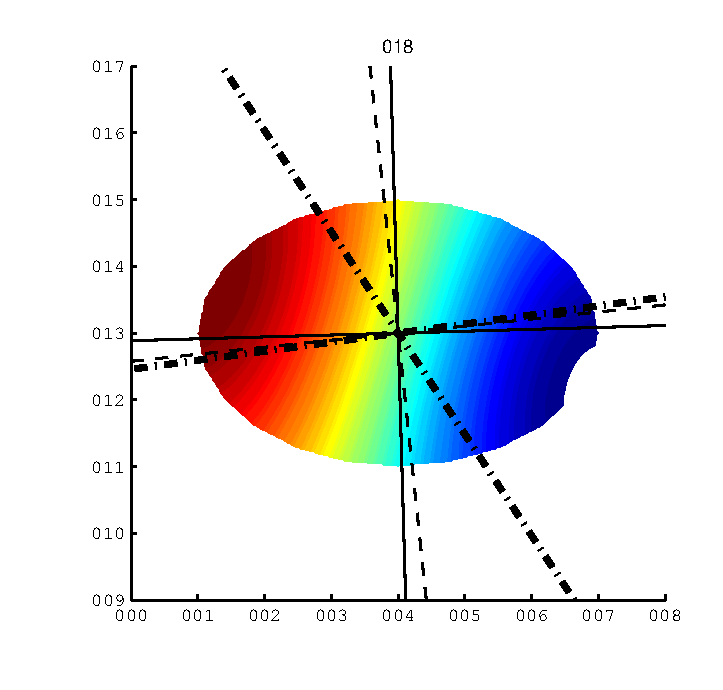
\includegraphics [width=0.22\linewidth ] {P_a_3_0kHz}

\vfill 

\makeatletter 
\immediate \write \@mainaux {\@percentchar </PSTOOLLABELS>}
\makeatother 
\end {document}

